\subsection*{Zadania: Siły wewnętrzne w belkach}

W poniższych układach wyznacz wykresy sił normalych, tnących oraz momentów zginających

\begin{figure}[htbp]
    \centering
    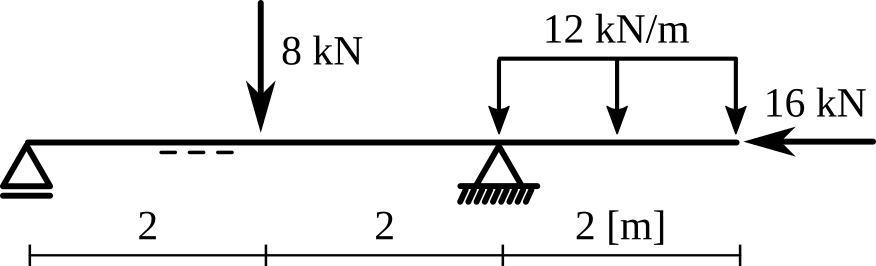
\includegraphics{Belki/Beam01.png}
    %\caption{}
\end{figure}

\begin{figure}[htbp]
    \centering
    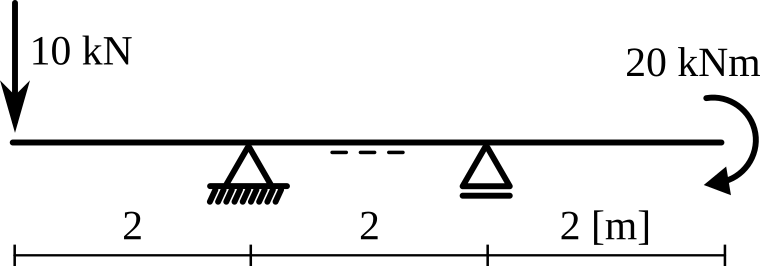
\includegraphics{Belki/Beam02.png}
    %\caption{}
\end{figure}

\begin{figure}[htbp]
    \centering
    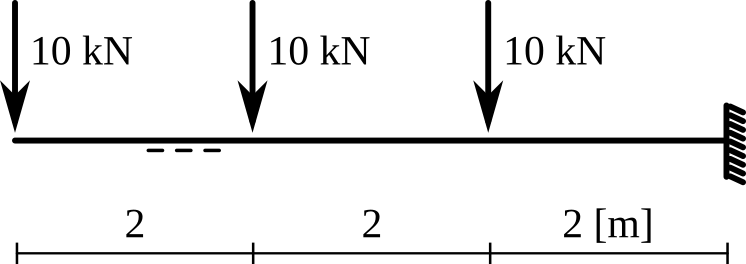
\includegraphics{Belki/Beam03.png}
    %\caption{}
\end{figure}

\begin{figure}[htbp]
    \centering
    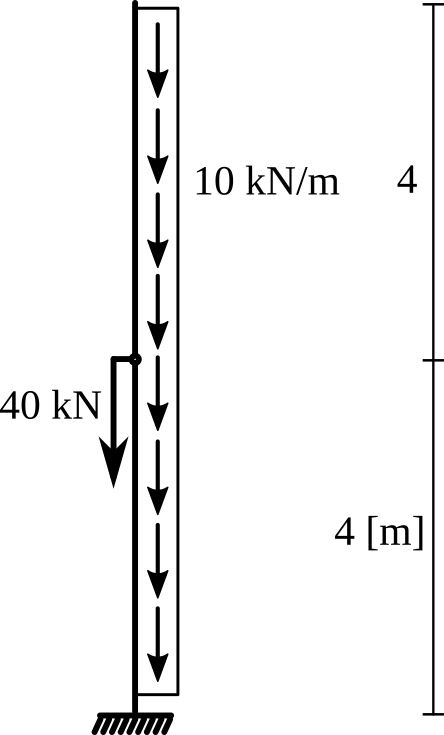
\includegraphics{Belki/Beam04.png}
    %\caption{}
\end{figure}